\documentclass[a4paper,11pt]{article}
  
\usepackage{graphicx}
\usepackage{amsmath}
\usepackage{array}
\usepackage{float}
\usepackage{subfigure}
\usepackage{color}
\usepackage{listings}
\usepackage[utf8x]{inputenc}
\usepackage{hyperref}
\usepackage{rotating}
\usepackage[english]{babel}

\usepackage{amsfonts,amsmath,amsthm,amssymb}
\usepackage{algorithm}
\usepackage{algpseudocode}

\renewcommand{\algorithmicrequire}{\textbf{Input:}}
\renewcommand{\algorithmicensure}{\textbf{Output:}}

%% --------- Algorithms -------------
\providecommand{\BeginAlgSize}[0]{\begin{scriptsize}}
\providecommand{\EndAlgSize}[0]{\end{scriptsize}}
\providecommand{\ForEach}[1]{\For{\textbf{each} #1}}
\providecommand{\Or}[0]{O}
\providecommand{\A}[0]{\mathbf{\alpha}}
%% --------- End of Algorithms -------------


% Read MRPT version:
\newread\file
\openin\file=../../version_prefix.txt
\read\file to\MRPTVERSION % Reads a line of the file 
\closein\file

% Title Page
\title{PbMap brief description and user guide.\\C++ implementation in \texttt{libmrpt-pbmap}}
\author{Eduardo Fern\'andez-Moral \\ efernandezmoral@gmail.com \\
%Jose-Luis Blanco-Claraco \\ joseluisblancoc@gmail.com \\
\\
\texttt{http://www.mrpt.org/} }
\date{MRPT version: \MRPTVERSION \\ Document build: \today }

% C++ listings settings
\lstset{ %
language=C++,                % choose the language of the code
basicstyle=\scriptsize,       % the size of the fonts that are used for the code
numbers=none,                   % where to put the line-numbers
numberstyle=\footnotesize,      % the size of the fonts that are used for the line-numbers
stepnumber=1,                   % the step between two line-numbers. If it is 1 each line will be numbered
numbersep=5pt,                  % how far the line-numbers are from the code
backgroundcolor=\color{white},  % choose the background color. You must add \usepackage{color}
commentstyle=\color{blue},
showspaces=false,               % show spaces adding particular underscores
showstringspaces=false,         % underline spaces within strings
showtabs=false,                 % show tabs within strings adding particular underscores
frame=single,           % adds a frame around the code
tabsize=2,          % sets default tabsize to 2 spaces
captionpos=b,           % sets the caption-position to bottom
breaklines=true,        % sets automatic line breaking
breakatwhitespace=false,    % sets if automatic breaks should only happen at whitespace
escapeinside={\%*}{*)}          % if you want to add a comment within your code
}

\begin{document}
\maketitle


\vfill

\begin{scriptsize}
\begin{center}

\includegraphics[width=3cm]{imgs/by-sa.pdf}
\\
This work is licensed under Attribution-ShareAlike 3.0 International (CC BY-SA 3.0) License.
\end{center}
\end{scriptsize}


\newpage
\tableofcontents
\newpage

\begin{figure}[t!]
    \begin{center}
    \begin{tabular}{cc}
		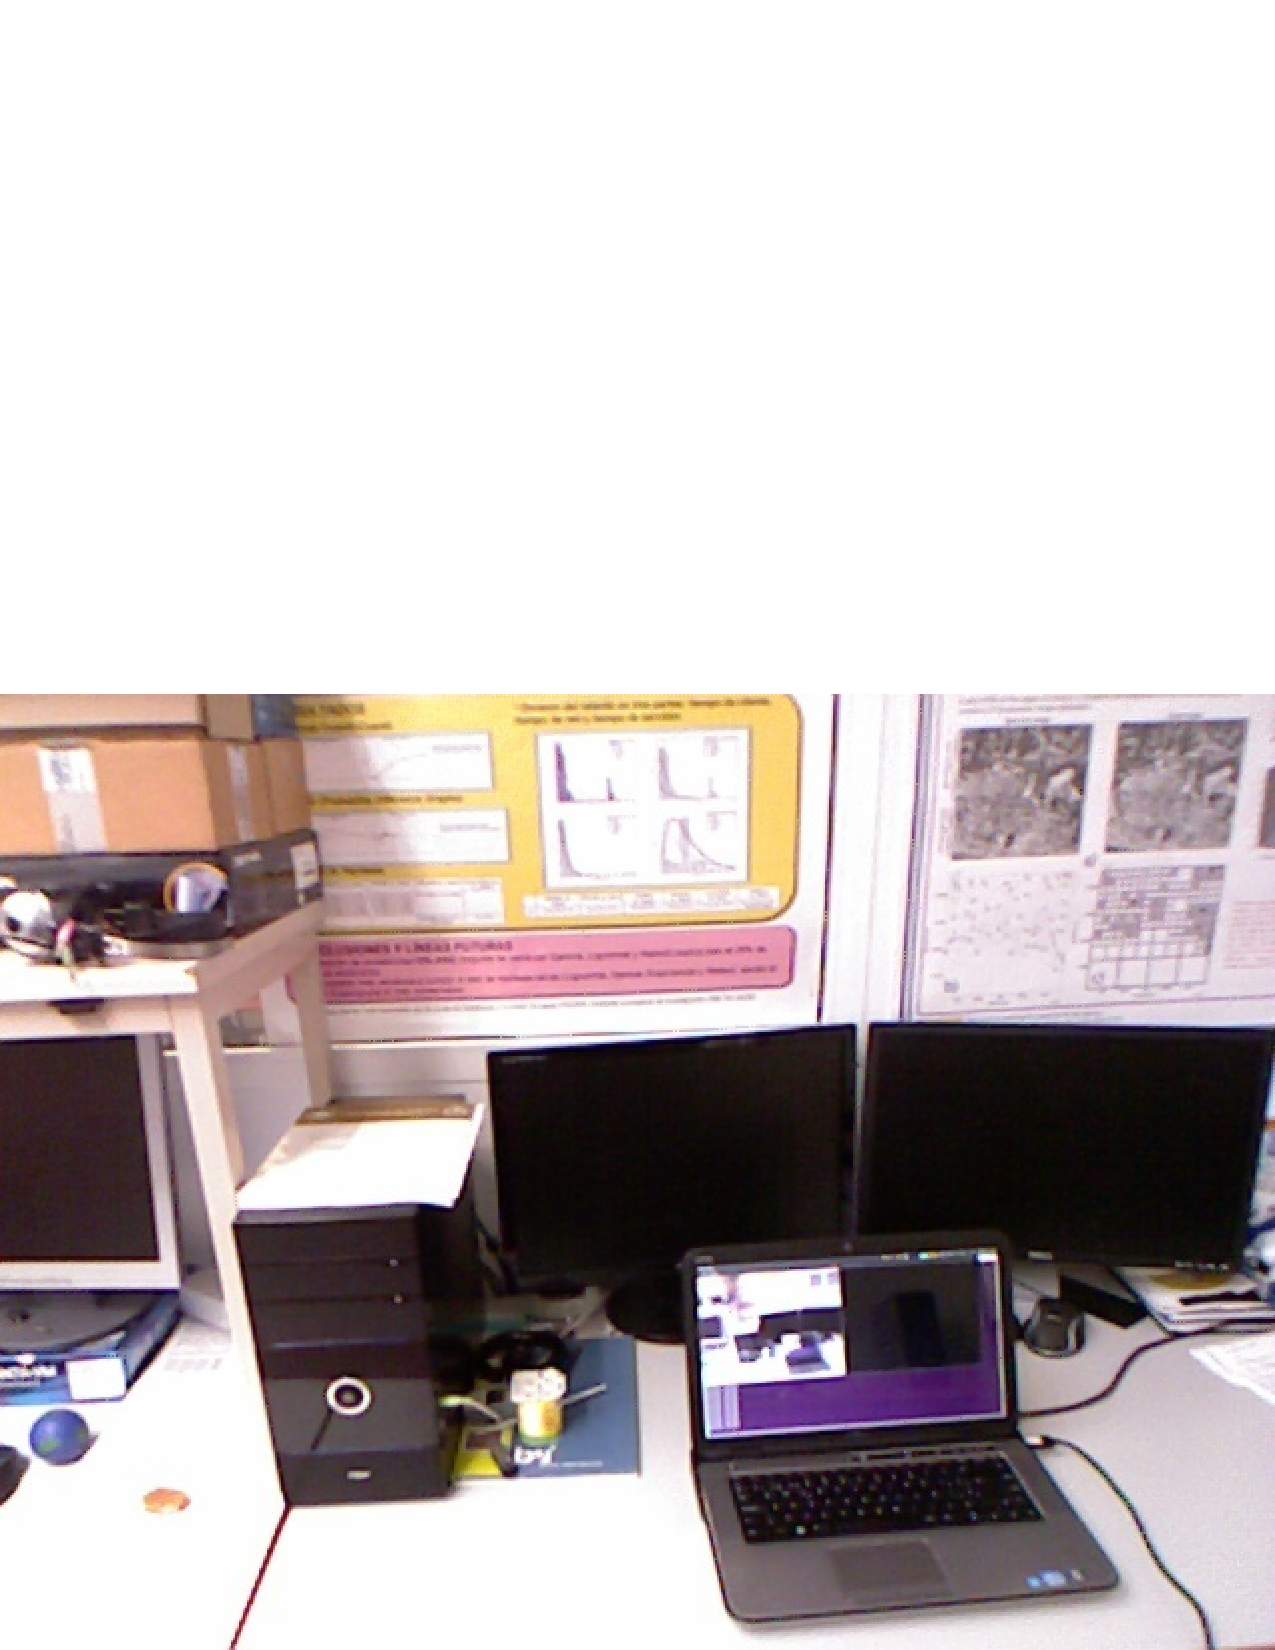
\includegraphics[width=0.42\textwidth]{imgs/scene.pdf} & 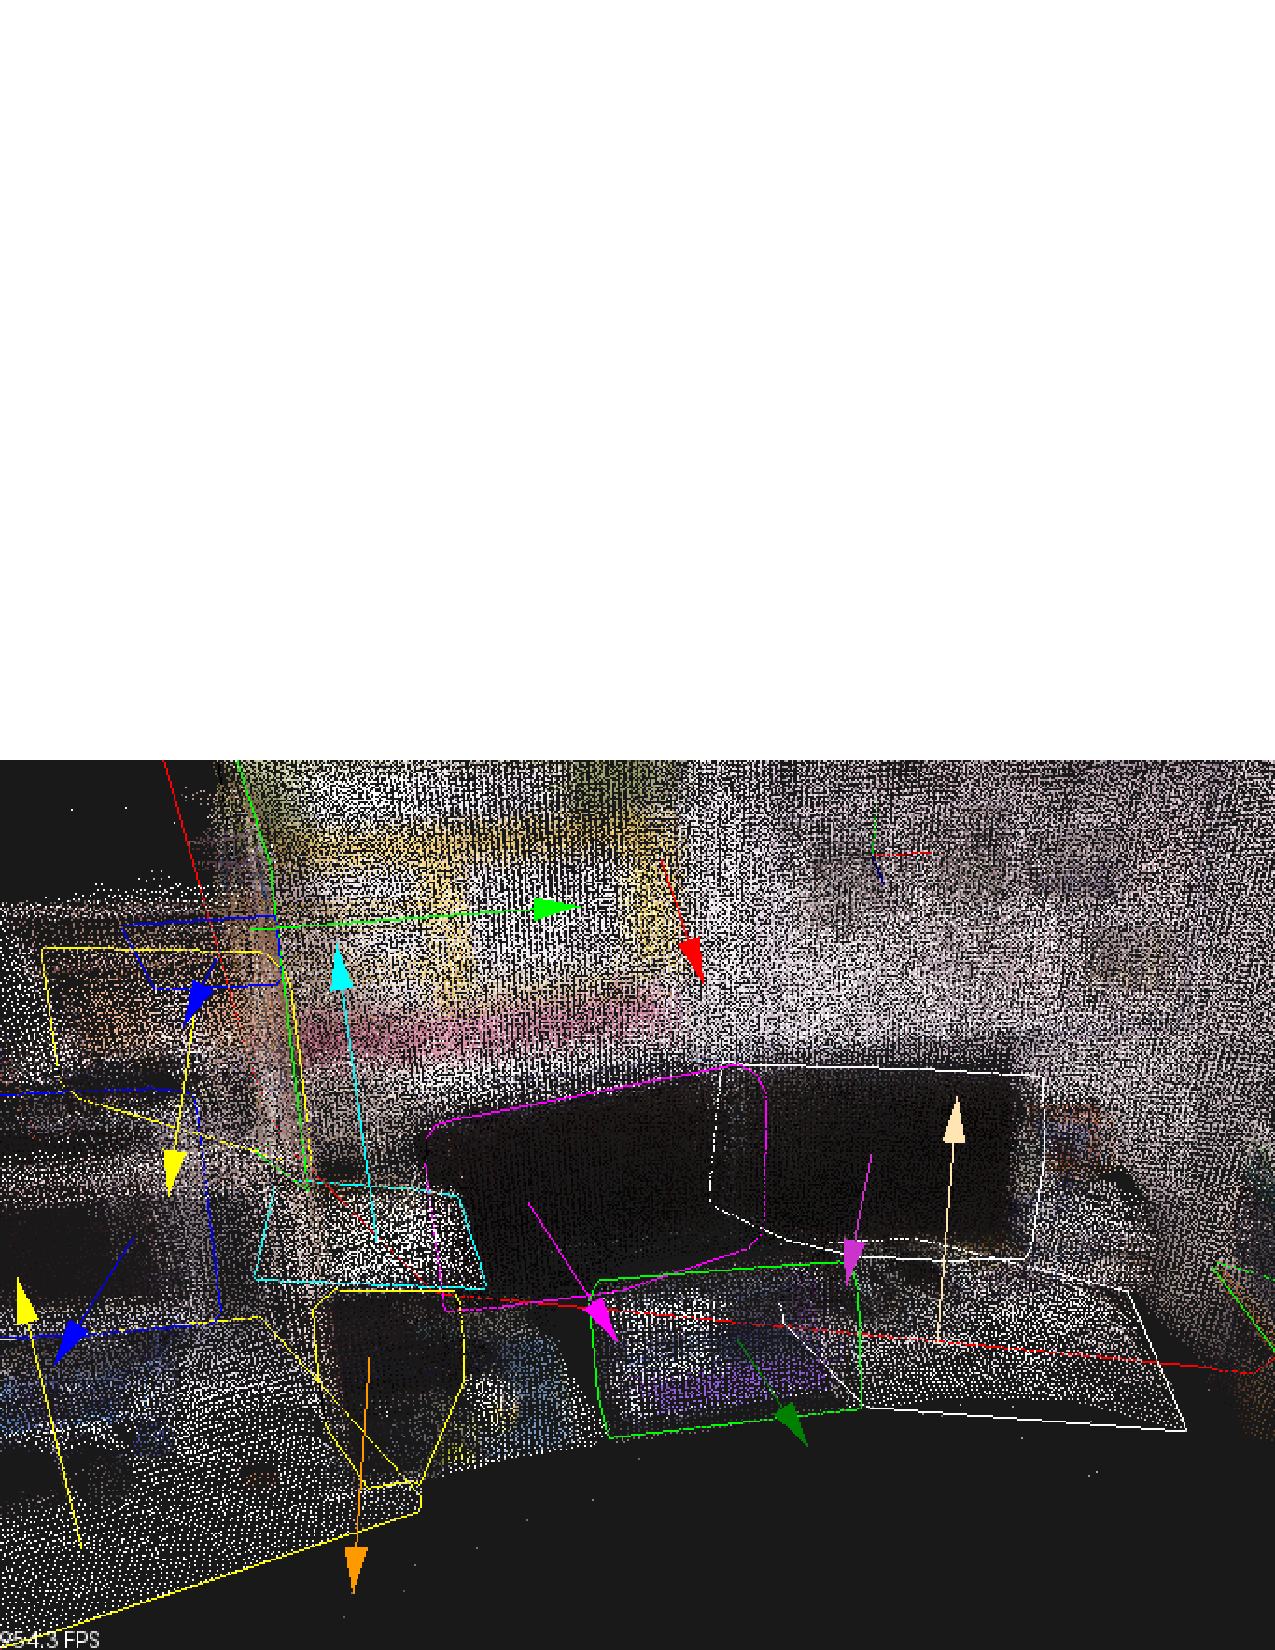
\includegraphics[width=0.45\textwidth]{imgs/pbmap.pdf} \\
		\scriptsize a) & \scriptsize b) \\
    \end{tabular}
    \end{center}
    \caption{Plane-based representation. a) RGB image of the scene. b) Point cloud representation with the segmented planar patches superimposed.}
	\label{fig:pbmap}
\end{figure}

\section{Introduction}

A PbMap is a highly compact representation of the scene based on a planar model of it. This map representation is proposed to avoid the high memory requirements and processing cost of traditional point cloud representations, which use has raised considerably with the appearance of low cost RGB-D (Kinect like) sensors. A PbMap compresses the point cloud into a set of planar patches, neglecting the non planar data. In this way, it offers an enormous data compression at the cost of losing the non-planar details, but we argue that such details have little importance for some applications, as for building lifelong maps, since only the large planes belonging to the scene structure are persistent over time, while the non-planar, generally small objects are more likely to move or disapear from the scene.

We define a PbMap as a set of planar patches described by geometric features (shape, relative position, etc.) and/or radiometric features (dominant color). It is organized as an annotated, undirected graph, where nodes stand for planar patches and edges connect neighbor planes when the distance between their closest points is under a threshold. This graph structure permits to find efficiently the closest neighbors of a plane, or to select groups of nearby planes representing part of the scene.

The input data to construct a PbMap is given by organized point clouds (depth images) together with poses. The process to build a PbMap can run online from the streaming of RGB-D images. This is possible thanks to efficient algorithms to segmentat planes from organized clouds \cite{holz2012fast}. The poses of those RGB-D images can be obtained in a number of ways: e.g. visual odometry, robot localization, etc. Thus, the planes are efficiently segmented from the organized point clouds, and these planes are  integrated into the PbMap according to the sensor pose, either by updating an already existing plane or by initializing a new one when it is first observed. Figure \ref{fig:pbmap_construction} depicts a 2D scheme of the PbMap construction process.

An application for recognising previous places using PbMaps is presented in \cite{fdez2013PbMap}. This method relies on an interpretation tree to efficiently match sets of neighboring planes. Such interpretation tree applies geometric and radiometric restrictions in the form of both unary and binary constraints \cite{grimson1990}. The unary constraints check the individual correspondence of two planes by comparing directly their features (e.g. size, color), while the binary constraints validate if two pairs of connected planes present the same geometric relationship (e.g. perpendicularity). For further details refer to our paper \emph{“Fast place recognition with plane-based maps”} \cite{fdez2013PbMap}. Some results of this work are shown in this video %\href{http://www.youtube.com/watch?v=uujqNm_WEIo}

\begin{figure}[t!]
  \centering
    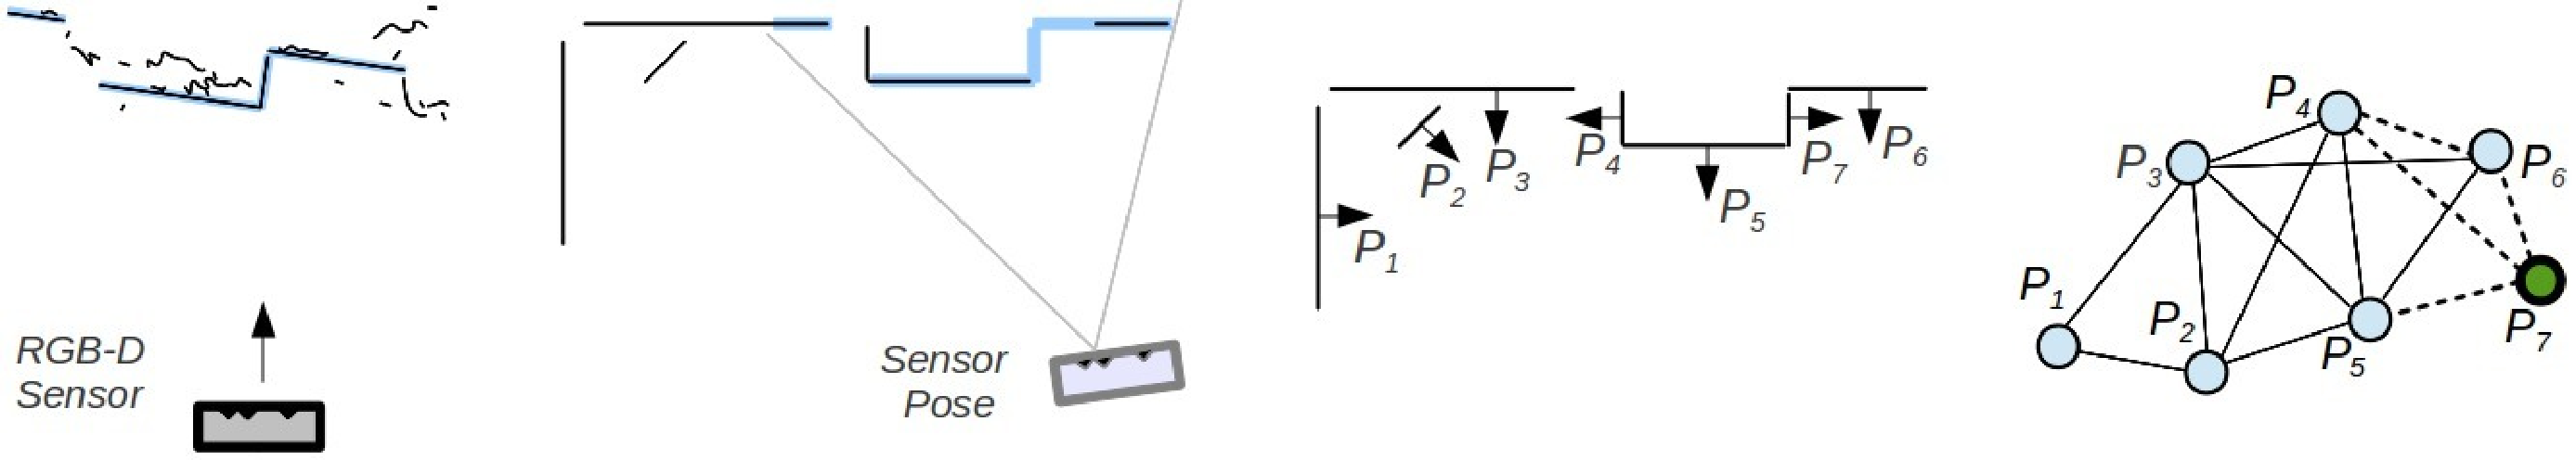
\includegraphics[width=1.0\textwidth]{imgs/pbmap_construction.pdf}
  \caption{2D representation of the map construction procedure. a) RGB-D capture with segmentated planes (blue). b) Current PbMap with segmented planes (blue) superimposed according to the sensor pose. c) PbMap updated: the planes updated are highlighted d) PbMap graph updated: the planes updated are highlighted in blue, the new plane P7 is marked in green and, the new edges are represented with dashed lines.}
  \label{fig:pbmap_construction}
\end{figure}

%\section{Library installation}
%

\section{Setting the parameters}

There are some heuristic parameters which govern the plane segmentation proces, the PbMap construction and the place recognition  and re-localisation methods. These parameters are set in two configuration files: \emph{configPbMap.ini} (for plane segmentation and PbMap construction) which is read by the class \texttt{PbMapMaker}; and \emph{configLocaliser.ini} (for place recognition and localisation) which is read by the class \texttt{heuristicParamenters}. Each parameter is described below: \\
 \\
\underline{Plane segmentation} (in \emph{configPbMap.ini})
\begin{itemize}
\item \emph{float dist\_threshold} → Set the maximum distance perpendicular to the plane between two 3D-points (default is set to 0.04 m).
\item \emph{float angle\_threshold} → Set the maximum angle between the normal vectors of two neighbor 3D-points (default is set to 4 deg).
\item \emph{float minInliersRate} → Set the minimum number of inliers as a fraction of the image pixels to segment a plane (default is set to 0.005).

\end{itemize}
\underline{Map construction} (in  \emph{configPbMap.ini}) \\
\\
\emph{Global settings:}
\begin{itemize}
\item \emph{bool use\_color} → Choose wether to add color information or not to the planes (default set to true);
\item \emph{int graph\_mode} → Choose between establishing edges in the graph according to distance (0) or to visibility (1) (default is set to 0);
\item \emph{float proximity\_neighbor\_planes} → Set the maximum distance between two planar patches to consider them as neighbors (default is set to 1 m);

\end{itemize}
\emph{Parameters to merge two planes representing the same planar surface:} 
\begin{itemize}
\item \emph{float max\_cos\_normal} → set the maximum angle (actually the minimum angle cosine) between two planes to merge them (default is set to 0.9848 = 10deg);
\item \emph{float max\_dist\_center\_plane} → Set the maximum distance between a plane and another plane's center to merge the planes (default is set to 0.1 m);
\item \emph{float proximity\_threshold} → Set the maximum distance between two planes to merge them (default is set to 0.15 m); 
\end{itemize}

\emph{Parameters to infer some simple semantic knowledge to the planar patches:}
\begin{itemize}
\item \emph{bool inferStructure} →  Choose wether to infer if the planes correspond to entities as e.g. floor, ceiling, walls, etc. (default is set to true);
\item \emph{bool makeCovisibilityClusters} → Should the PbMapMaker cluster groups of planes according to their co-visibility (default is set to true);

\end{itemize}
\emph{Loop closure:}
\begin{itemize}
\item \emph{bool detect\_loopClosure} → If set to true it runs the PbMapLocaliser functionality in a different thread to detect loop closures or to recognise previous PbMaps (default is set to true)
\item \emph{string config\_localiser} → Path to the configuration file containing the heuristic parameters which control the place recognition functionality;
\\

\end{itemize}
\underline{Place recognition} (in \emph{configLocaliser.ini}) *These parameters are required only if detect\_loopClosure=true \\
\\
\emph{Global settings:}
\begin{itemize}
\item \emph{string path\_prev\_pbmaps} → Path to previous PbMaps which are to be detected while cunstructing the current PbMap;
\item \emph{int min\_planes\_recognition} → Minimum number of planes to accept a match between two places (defaultis is set to 4);
\item \emph{bool use\_structure} → Choose whether to employ or not the semantic knowledge inferred to the planes (default is set to true);
\item \emph{use\_completeness} → Choose whether to differentiate between fully detected planes and partial observations to set different constraints for matching planes (default set to true);

\end{itemize}
\emph{Unary constraints:}
\begin{itemize}
\item \emph{color\_threshold} → Maximum color difference to match two planes (default set to 0.1);
\item \emph{elongation\_threshold} → Maximum elongation ratio to match two planes ratio (default set to 2.8)     
\item \emph{area\_threshold} → Maximum areas ratio to match two planes (default set to 3.0)	              
\item \emph{area\_full\_threshold} → Used only if use\_completeness is true. Maximum areas ratio to match two planes (default set to 3.0);
\item \emph{area\_half\_threshold} → Used only if use\_completeness is true. Maximum areas ratio to match two planes (default set to 2.5);

\end{itemize}
\emph{Binary constraints:}
\begin{itemize}
\item \emph{angle\_threshold} → Maximum difference between the angles formed by of two pairs of planes to match such pairs (default set to 7.0)
\item \emph{dist\_threshold} → Maximum ratio between the distances of two pairs of planes to match such pairs (default set to 2.0)
\item \emph{height\_threshold} → Maximum difference between the height of two pairs of planes (almost parallel) to match such pairs (default set to 0.2 m)
\item \emph{cos\_angle\_parallel} → Maximum angle difference to consider two planes almost parallel (default set to 0.985)
\end{itemize}


%\section{Programmer's first steps}
%\label{sect:program_first}

\section{Implementation in MRPT (lib \texttt{mrpt-pbmap})}
\label{sect:implementation}

This library implements the functionality to build Plane-based Maps (PbMaps) from a set of point clouds plus their corresponding poses, which might be given by e.g. the odometry of a robot.
Application examples

Two application examples have been created for creating PbMaps \\ (\texttt{pbmap\_example}) and for visualising them (\texttt{pbmap\_visualizer}). To build the example within MRPT, the Cmake option BUILD\_EXAMPLES must be set to ON (default is OFF).

\subsection{How to create a simple program to build a PbMap}

The central class in mrpt-pbmap is PbMapMaker. This class creates its own thread in which it runs. The input data is passed through its public member frameQueue which stores a vector of pairs of point cloud plus pose. Thus, in order to create a PbMap, the user just need to create an object PbMapMaker and fill the vector frameQueue:

\begin{lstlisting}
#include <mrpt/pbmap.h>

using namespace mrpt::pbmap;
using namespace std;

int main(int argc, char**argv)
{
	//  Create a PbMapMaker object specifying the configPbMap.ini
	PbMapMaker pbmap_maker("path_to/config_files/pbmap/configPbMap.ini"); 
	
	// While certain condition is fulfilled (e.g. while exploration)
	while (...) {
		...

		// Get dupla point_cloud + pose
		frameRGBDandPose cloudAndPose;
		pcl::copyPointCloud(point_cloud, *cloudAndPose.cloudPtr);
		cloudAndPose.pose << pose;

		// Detect planes and build PbMap
		pbmap_maker.frameQueue.push_back(cloudAndPose);

		...
	}
}
\end{lstlisting}

Also, loop closure is run if it was activated in the configuration file  configPbMap.ini. Note that we treat loop closure and place recognition in an equivalent manner, with the only difference that place recognition implies searching previous PbMaps with yet no relation with the current one being built.


%% ---------------------------------------------------------------
%%                         BIBLIOGRAPHY
%% ---------------------------------------------------------------
%\newpage
\bibliographystyle{plain}
\bibliography{cites}

\end{document}

